% Pollo al Curry
\newpage
%\thispagestyle{empty}
\begin{recipe}[source={Propia},
portion={4-6 porciones},
preparationtime={\unit[20]{Minutos}}
]{Pollo al curry}
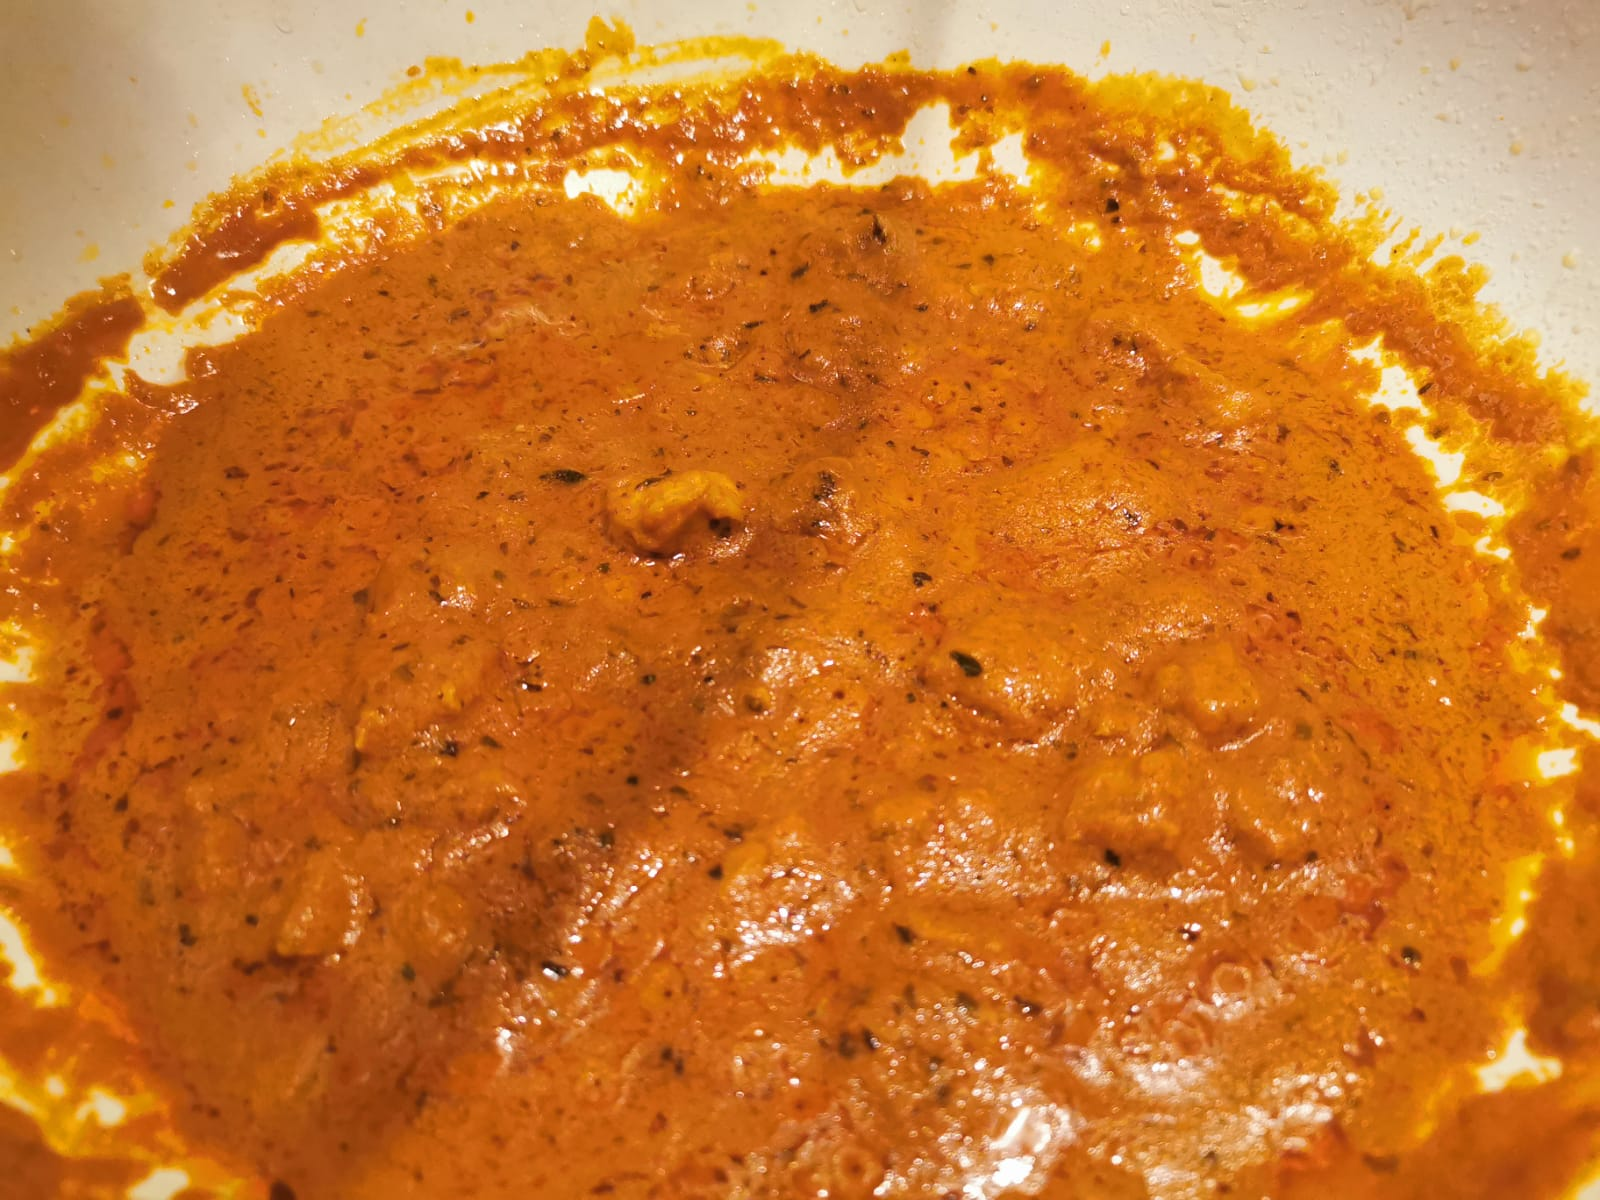
\includegraphics[width=0.25\textwidth]{pollo-curry}
\introduction{
Esta es una receta nueva, vi una similar en algun recetario pero la adapté a mi paladar.
}
\ingredients{
    1 & Pechuga de pollo deshuesada cortada en cubitos pequeños \\
    1 & Cebollas cortadas finamente en cuadritos \\
    3 & Dientes de ajo picados \\
    & Orégano a gusto \\
    1 & Salsa de tomate o tomate triturado \\
      & Aceite de oliva \\
      & Sal \\
      & Pimienta \\
    2 & Cucharadas de curry \\
    1 & Tarro de crema de leche
}
\preparation{
    \begin{enumerate}
        \item Aliñar o salpimentar el pollo con la sal y pimienta.
        \item En una sartén, agregar un poco de aceite y calentar a fuego fuerte.
        \item Cuando el aceite esté listo, agregar el pollo y dejar sellar por un lado por aproximadamente 2 minutos, luego mover para dorar el resto del pollo por aproximadamente el mismo tiempo.
        \item Agregar la cebolla, el ajo, el orégano y preparar el sofrito.
        \item Cuando la cebolla esté traslucida, agregar el curry y revolver un poco.
        \item Agregar la salsa de tomate o el tomate triturado y revolver un poco.
        \item Agregar la crema de leche y revolver hasta que todo esté integrado.
        \item Dejar a fuego lento y revolver de cuando en vez por aproximadamente 15 minutos.
        \item transcurrido el tiempo, retirar y servir.
    \end{enumerate}
}
\hint{
	Se puede acompañar con arroz o pastas.
}
\end{recipe}